\section{More Examples of Data Flow Analysis: Global Common Sub-expression Elimination; Constant Propagation/Folding}

If we care about the past, what happened before, then it is a forward problem (entry). 


\subsection{Available Expression Analysis}


\begin{definition}{Availability of an Expression E at point P}
E is available at P if every path to P in the flow graph
\begin{itemize}
    \item E must be calculated at least once
    \item no variable in E redefined after the last evaluation

\end{itemize}
\end{definition}


\begin{figure}[h]
    \centering
    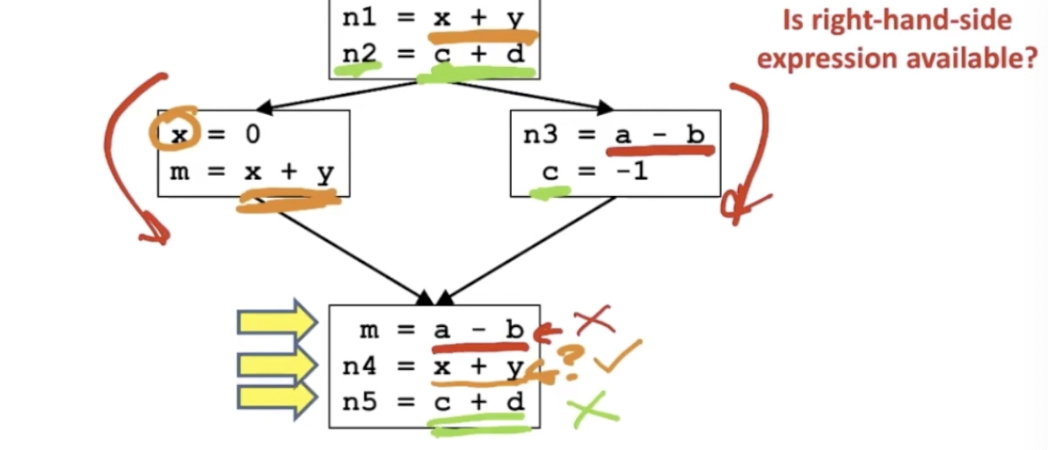
\includegraphics[width=0.3\textwidth]{p24.png}
    \caption{}
    \label{fig:p24}
\end{figure}


\subsubsection{Examples}



In \ref{fig:p24} $a-b$, $c+d$ is not available at the last BB. But $x+y$ is.


\begin{figure}[h]
    \centering
    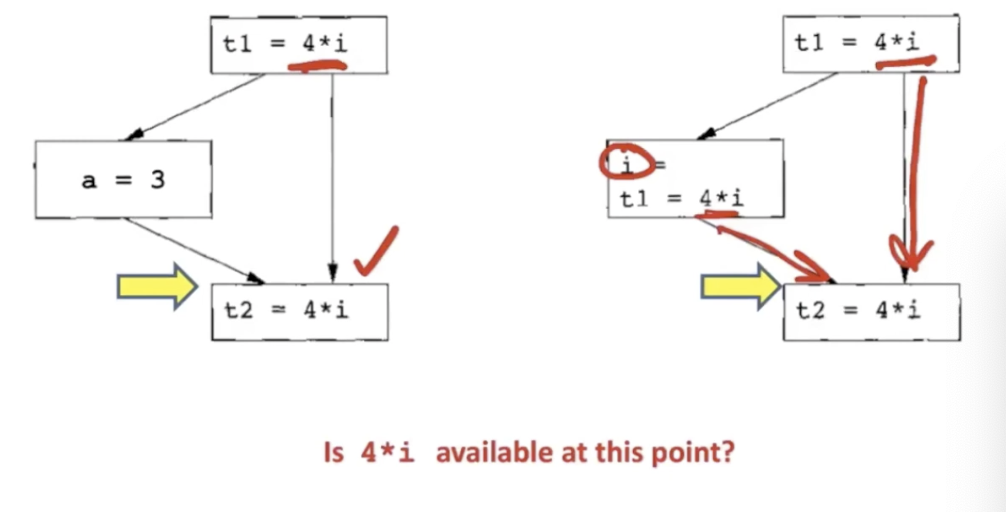
\includegraphics[width=0.3\textwidth]{p25.png}
    \caption{}
    \label{fig:p25}
\end{figure}


In \ref{fig:p25} , $4*i$ is available for both cases.



\begin{figure}[h]
    \centering
    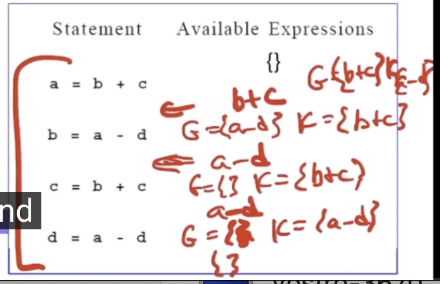
\includegraphics[width=0.3\textwidth]{p26.png}
    \caption{}
    \label{fig:p26}
\end{figure}


In \ref{fig:p26}, we show that calculate transfer functions for complete basic blocks by composing individual instruction transfer functions.


\begin{figure}[h]
    \centering
    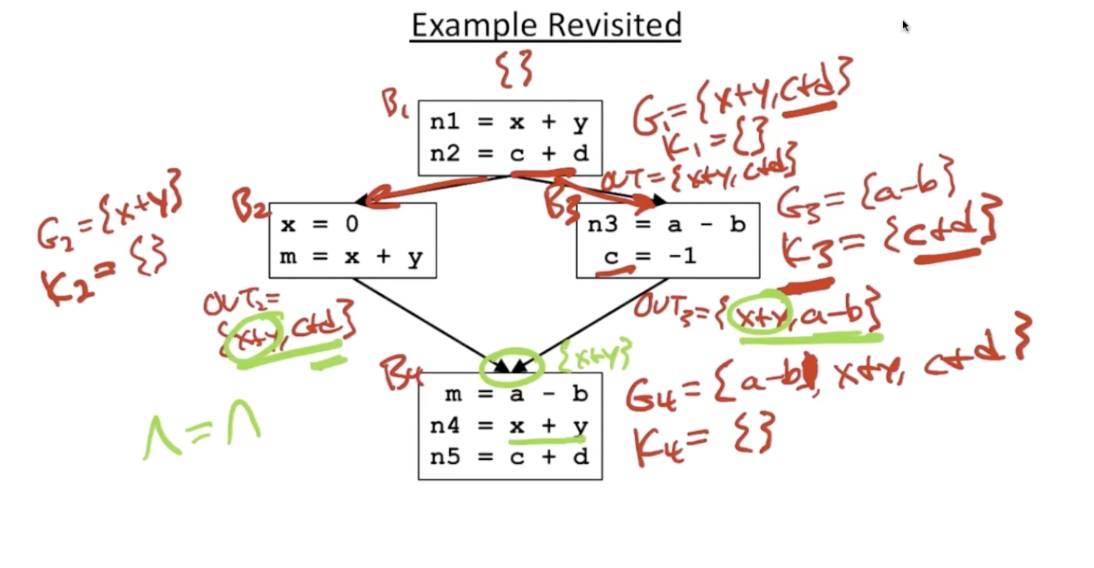
\includegraphics[width=0.3\textwidth]{p27.png}
    \caption{}
    \label{fig:p27}
\end{figure}


\subsection{Eliminating CSEs}


\begin{itemize}
    \item Step1: Value Numbering
    \item Step2: Available expression
    \item Step3: If CSE is an "available expression", then transform the code.
    
\end{itemize}

\begin{figure}[h]
    \centering
    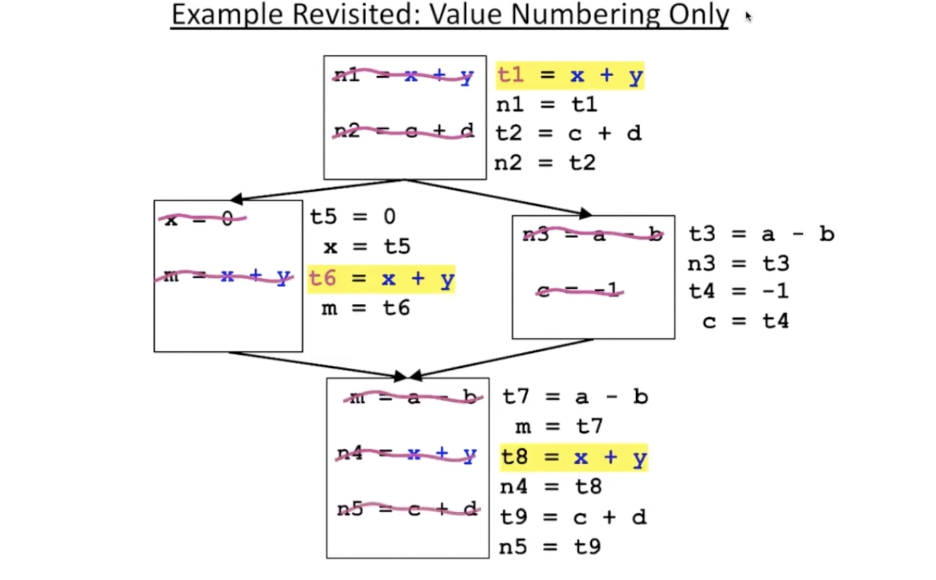
\includegraphics[width=0.3\textwidth]{p28.png}
    \caption{}
    \label{fig:p28}
\end{figure}

If we only use value numbering to eliminate common expression in \ref{fig:p28}, we will see that this will just add a lot of new work and no income. But if we calculate Available expression in \ref{fig:p29}, we can find that $x+y$ is such one and can do some optimization.


\begin{figure}[h]
    \centering
    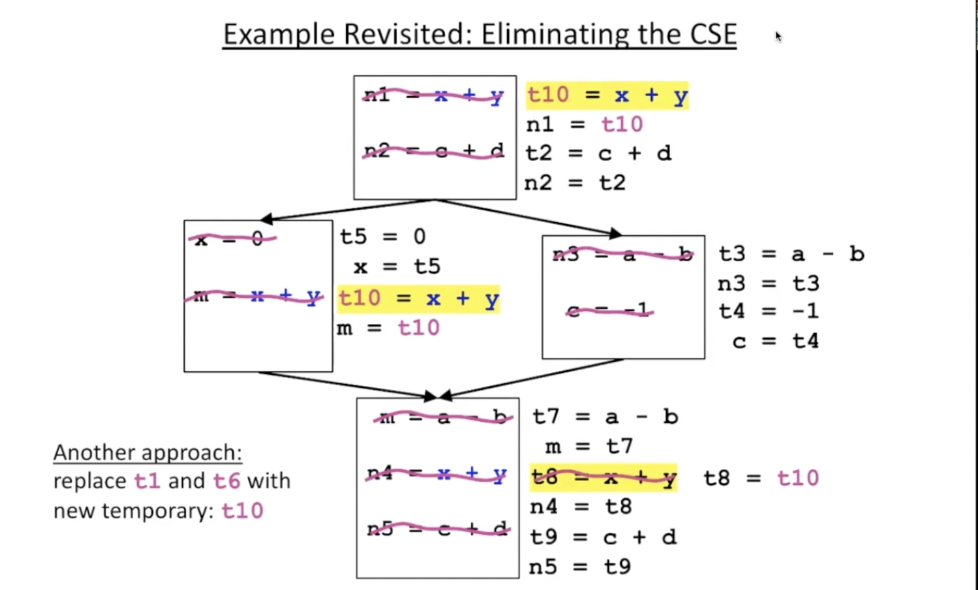
\includegraphics[width=0.3\textwidth]{p29.png}
    \caption{}
    \label{fig:p29}
\end{figure}

\begin{note}{How to deal with Textually identical expression?\ref{fig:p30}}
Just sort the operands.



But for textually different expressions that may be equivalent \ref{fig:p31}, we had better do copy propagation first.

\end{note}
\begin{figure}[h]
    \centering
    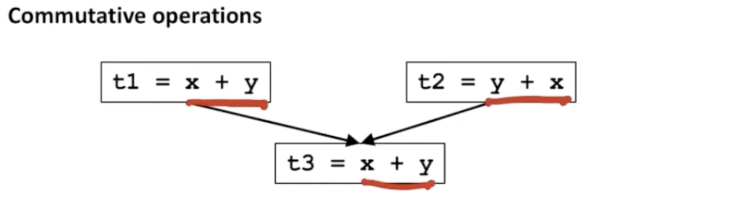
\includegraphics[width=0.3\textwidth]{p30.png}
    \caption{}
    \label{fig:p30}
\end{figure}

\begin{figure}[h]
    \centering
    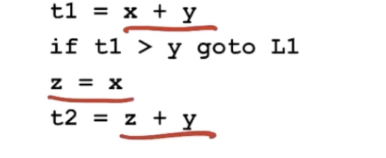
\includegraphics[width=0.3\textwidth]{p31.png}
    \caption{}
    \label{fig:p31}
\end{figure}


\subsubsection{Summary}

\begin{figure}[h]
    \centering
    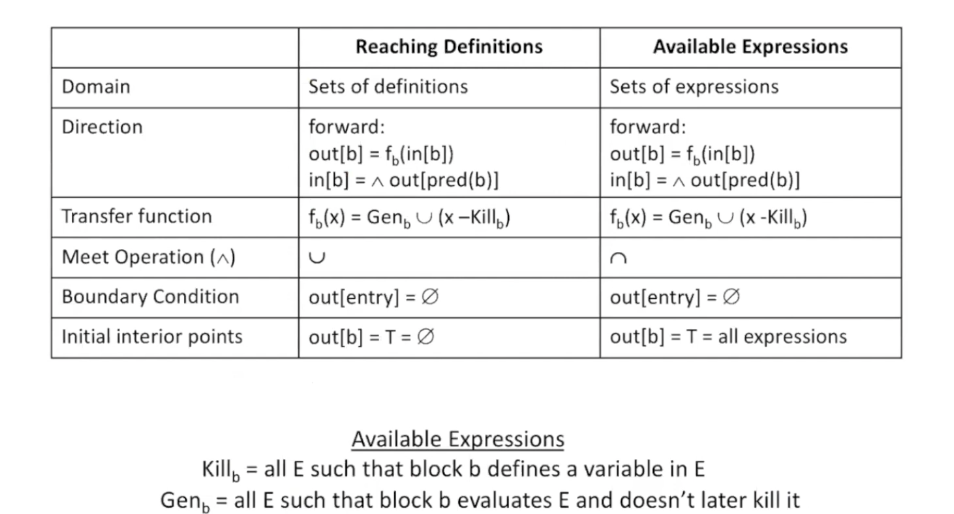
\includegraphics[width=0.3\textwidth]{p32.png}
    \caption{}
    \label{fig:p32}
\end{figure}


\subsection{Constant Propagation/Folding}

\begin{figure}[h]
    \centering
    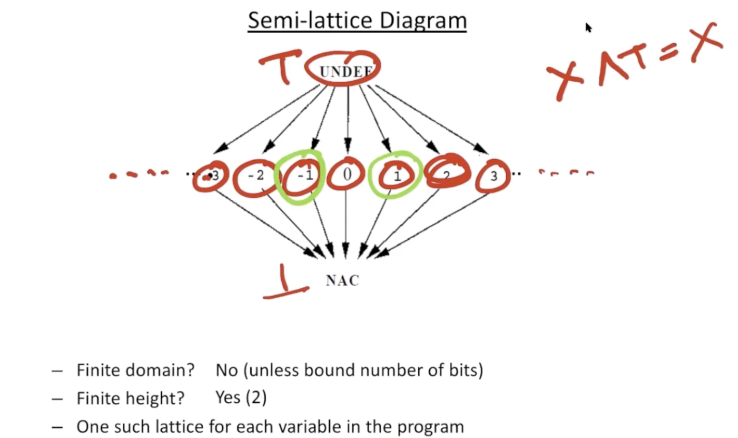
\includegraphics[width=0.3\textwidth]{p33.png}
    \caption{}
    \label{fig:p33}
\end{figure}

\subsubsection{Meet Operator in Table Form}
\begin{figure}[h]
    \centering
    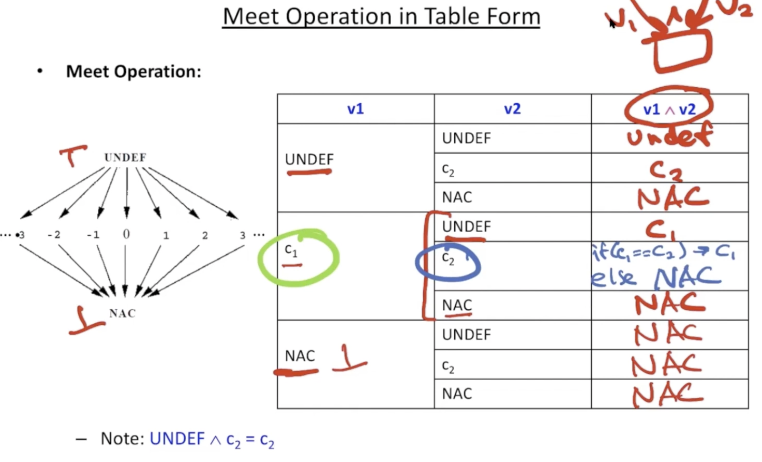
\includegraphics[width=0.3\textwidth]{p34.png}
    \caption{}
    \label{fig:p34}
\end{figure}


\subsubsection{Example}

\begin{figure}[h]
    \centering
    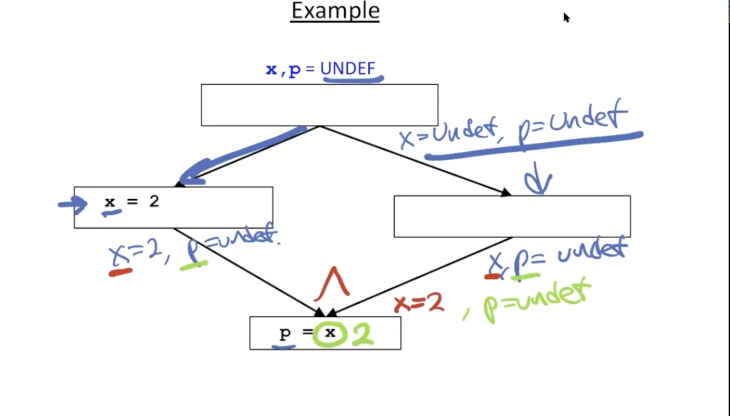
\includegraphics[width=0.3\textwidth]{p35.png}
    \caption{}
    \label{fig:p35}
\end{figure}

On the other path in \ref{fig:p35}, x is uninitialized. When we have undefined behavior, hopefully the front end of the compiler should complain about it, but if it doesn't, the optimizer is free to do whatever it wants to do.


\subsubsection{Transfer Function}


\begin{figure}[h]
    \centering
    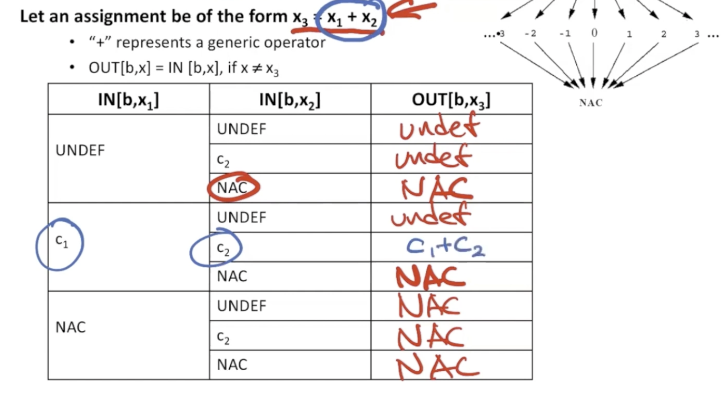
\includegraphics[width=0.3\textwidth]{p36.png}
    \caption{}
    \label{fig:p36}
\end{figure}



It is not distributive in \ref{fig:p37}.

\begin{figure}[h]
    \centering
    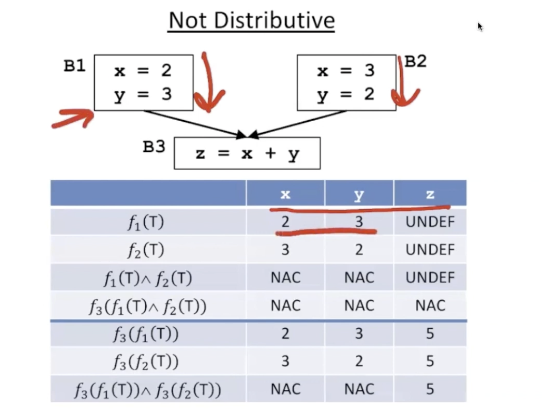
\includegraphics[width=0.3\textwidth]{p37.png}
    \caption{}
    \label{fig:p37}
\end{figure}



\subsection{Copy Propagation}

\subsection{Dead Code Elimination}

